\documentclass{article}
\usepackage[fleqn]{amsmath}
\usepackage{amssymb,graphicx,color,graphicx,slashed, microtype, parskip, enumitem, extarrows, needspace}
%\usepackage[utf8x]{inputenc}
\usepackage[top=1.5cm, bottom=1.5cm, right=6cm, left=1.5cm, heightrounded, marginparwidth=5cm, marginparsep=0.5cm]{geometry}

\hbadness = 10000
\hfuzz=100pt 
    
\usepackage{marginnote}
\renewcommand*{\marginfont}{\footnotesize}

\usepackage{hyperref}
\hypersetup{colorlinks=true, urlcolor=NavyBlue, bookmarksdepth=3}

\makeatletter\newcommand{\@minipagerestore}{\setlength{\parskip}{\medskipamount}}\makeatother

% =============== Index ===========================

\usepackage[nonewpage]{imakeidx}
\makeindex

% =============== Color Definitions ===============
    
\usepackage[svgnames]{xcolor}
\colorlet{ColorTitle}{Black}
\colorlet{ColorSectionName}{Black}
\colorlet{ColorBoxFG}{Gray}
\colorlet{ColorBoxText}{Black}
\colorlet{ColorBoxBG}{White}


% =============== Title Style ===============
    
\usepackage{titling} % Allows custom title configuration
    
\newcommand{\HorRule}{\color{ColorTitle}\rule{\linewidth}{1pt}} % Defines the gold horizontal rule around the title
    
\pretitle{
    \vspace{-50pt} % Move the entire title section up
    \HorRule\vspace{9pt} % Horizontal rule before the title
    \fontsize{27}{36}\usefont{OT1}{phv}{b}{n}\selectfont
    \color{ColorTitle} % Text colour for the title and author(s)
}
    
\posttitle{\par\vskip 15pt} % Whitespace under the title
    
\preauthor{\fontsize{17}{0}\usefont{OT1}{phv}{m}{n}\selectfont\color{ColorTitle}} % Anything that will appear before \author is printed
    
\postauthor{\par\HorRule}

\newcommand{\COURSENAME}{\href{http://phyw.people.ust.hk/teaching/PHYS2022-2015/}{\textcolor{black}{PHYS 2022}}}
\newcommand{\YW}{\href{http://phyw.people.ust.hk/}{\textcolor{black}{Yi Wang}}}
\newcommand{\PHYS}{\href{http://physics.ust.hk}{\textcolor{black}{Department of Physics}}}
\newcommand{\HKUST}{\href{http://www.ust.hk/}{\textcolor{black}{HKUST}}}
\author{\COURSENAME, \YW, \PHYS, \HKUST}

\date{}

% =============== Section Name Style ===============
    
\usepackage{titlesec}
    
\titleformat{\section}
    {\fontsize{15}{20}\usefont{OT1}{phv}{b}{n}\color{ColorSectionName}}
    {\thesection}{1em}{}
    %[{\vspace{0.2cm}\titlerule[0.8pt]}]
    
\titleformat{\subsection}
    {\fontsize{14}{20}\usefont{OT1}{phv}{m}{n}\color{ColorSectionName}}
    {\thesubsection}{1em}{}
    
\titleformat{\subsubsection}
    {\fontsize{12}{20}\usefont{OT1}{phv}{m}{n}\color{ColorSectionName}}
    {}{0em}{}
      
\setcounter{secnumdepth}{4}
        
% =============== Box Style ===============
    
\usepackage[most]{tcolorbox}
    
\newtcolorbox{tbox}[1]{
    colback=ColorBoxBG, colframe=ColorBoxFG, coltext=ColorBoxText,
    sharp corners, enhanced, breakable, parbox=false,
    before skip=1em, after skip=1em,
    title={#1}, fonttitle=\usefont{OT1}{phv}{b}{n}, 
    attach boxed title to top left={yshift=-0.1mm}, boxed title style={sharp corners, colback=ColorBoxFG, left=0.405cm},
    rightrule=-1pt,toprule=-1pt, bottomrule=-1pt
}

\newtcolorbox{mtbox}[1]{
    colback=ColorBoxBG, colframe=ColorBoxFG, coltext=ColorBoxText,
    sharp corners, enhanced, breakable, parbox=false,
    before skip=1em, after skip=1em,
    title={#1}, fonttitle=\usefont{OT1}{phv}{b}{n},
    attach boxed title to top left={yshift=-0.1mm}, boxed title style={sharp corners, colback=ColorBoxFG, left=0.15cm},
    rightrule=-1pt,toprule=-1pt, bottomrule=-1pt, 
    left=0.5em
}

% =============== tikz has to be loaded after xcolor
\usepackage{tikz}

\newcommand*\enumlabel[1]{\tikz[baseline=(char.base)]{
			\node[shape=rectangle,inner sep=2pt,fill=ColorBoxFG] (char) 
			{\fontsize{7}{20}\usefont{OT1}{phv}{b}{n}{\textcolor{ColorBoxBG}{#1}}};}}

% =============== Useful shortcuts ===============

\newcommand\wref[1]{{\hypersetup{linkcolor=white}\ref{#1}}}  

\newcommand{\textbox}[2]{
    \begin{tbox}{#1}
        #2
    \end{tbox}
}

\newcommand{\mtextbox}[2]{\marginnote{
    \begin{mtbox}{#1}
        #2
    \end{mtbox}}
}

\newcommand{\mnewline}{\vspace{0.5em}\newline}

\newcommand{\titem}[1]{
    \begin{itemize}[label=\color{ColorBoxFG}$\blacktriangleright$, leftmargin=0mm, labelsep=0.27cm, topsep=0.5em
        %, itemsep=1ex
        ]
        #1
    \end{itemize}
}

\newcommand{\mtitem}[1]{
    \begin{itemize}[label={\color{ColorBoxFG}$\blacktriangleright$}, leftmargin=0mm, labelsep=1mm, topsep=0.5em
        %, itemsep=1ex
        ]
        #1
    \end{itemize}
}

\newcommand{\itembox}[3]{
    \begin{tbox}{#1}
        #2
        \titem{#3}
    \end{tbox}
}

\newcommand{\mitembox}[3]{
    \marginnote{
    \begin{mtbox}{#1}
        #2
        \mtitem{#3}
	\end{mtbox}
    }
}

\newcommand{\tenum}[1]{
    \begin{enumerate}[label=\protect\enumlabel{\arabic*}, leftmargin=0mm, labelsep=0.265cm, topsep=0.5em
        %, itemsep=1ex
        ]
        #1
    \end{enumerate}
}

\newcommand{\enumbox}[3]{
    \begin{tbox}{#1}
        #2
        \tenum{#3}
    \end{tbox}
}

\newcommand{\twocol}[5]{
    \begin{minipage}[t][][b]
        {#1\textwidth}
        #4        
    \end{minipage}
    \hspace{#2\textwidth}
    \begin{minipage}[t][][b]
        {#3\textwidth}
        #5
    \end{minipage}
}

\newcommand{\cg}[2]{
    \begin{center}
        \includegraphics[width=#1\textwidth]{#2}
    \end{center}
}

\newcommand{\tbar}{
    ~\newline
    {\color{ColorBoxFG}
    \hbox to 0.15\textwidth{\leaders\hbox to 5pt{\hss  \hss}\hfil} 
    \hbox to 0.7\textwidth{\leaders\hbox to 5pt{\hss . \hss}\hfil}}
    \mnewline
}

% =============== Filter unwanted warnings
\usepackage{silence}
\WarningsOff[tcolorbox]
\hbadness=1000000


\usepackage{5_fig/modiagram}
\graphicspath{{5_fig/}}
\title{Part 5. Atoms}

\begin{document}

\maketitle

\textbox{Feynman's question}{
    As the opening of his lectures, Feynman asked the following question:
    \begin{quote}
        If, in some cataclysm, all of scientific knowledge were to be destroyed, and only one sentence passed on to the next generations of creatures, what statement would contain the most information in the fewest words? 
    \end{quote}
    He gave an answer himself:
    \begin{quote}
        Matter is made of atoms.
    \end{quote}
    This statement is not absolutely right. For example, E\&M waves may be considered a form of matter which is not made of atoms (though made of quanta). Dark matter is not made of conventional atoms either, and dark energy does not look like atoms by all means. Nevertheless, our familiar matter world is indeed made of atoms. 
    \marginnote{
        With modern technology, \ref{item:atom-chem}, \ref{item:atom-size} and \ref{item:atom-evid} seems trivial. Because scanning tunneling microscopes can directly see and manipulate atoms. However, back to 150$\sim$200 years ago, how these features were known from scientific methods? Strictly speaking, they are not part of modern physics. But as it is not completely covered in general physics, I decide to include it here.
    }
    And I agree that this is the message that we should pass on. 
    \tcblower
    How do we know, why do we care, and what are the consequences that the world is made of atoms? This will be the focus of this part. More explicitly, we will address:
    \tenum{
        \item How the atomic theory arised in chemistry?\label{item:atom-chem}
        \item How do we know the size of an atom?\label{item:atom-size}
        \item Can we find direct evidences for the existence of atoms?\label{item:atom-evid}
        \item How can an atom be stable? -- How does quantum mechanics save the world?\label{item:atom-quantum}
        \item Where do the chemical natures of atoms arise?\label{item:atom-chem-nature}
    }
    \mtextbox{Oil film method}{
        Independently, the size of atoms (molecules) can also be determined by oil film method. Franklin (1757) noted that oil can spread on a huge area of water. The thin film of oil upon water can be as thin as a single layer of molecule. However, such huge area is hard to measure. Is it possible to make the amount of oil smaller?
        \tcblower
        Langmuir (1917) used alcohol to dissolve oleic acad. Drip one drop of such solution to water. Alcohol is dissolved by water and oleic acad spread on the surface of water with an area measurable in a lab.
    }
}

\section{How did we know that matter is made of atoms?}

The atomic theory was proposed by the ancient Greece (and other cultures) over 2000 years ago. However, at that time the atomic theory is based on philosophical guess and has little scientific support. The scientific atomic theory starts from the 19th century. 

\textbox{Dalton's law of multiple proportions\index{Dalton's multiple proportion law}}{
    Dalton (1808) noted that carbon can combine with oxygen in two different ways to form oxides. For fixed amount of carbon, the amount of oxygen needed in these two oxides is 1:2 -- a ratio constitute of two small integers. 

    Is this observation a coincidence? Dalton tested other pairs of elements (which can form at least two different compounds). Similar properties are noted: Fixing the amount of one element, the amount of the other element needed for different compounds are ratios with small integers.
    \tcblower
    Such an observation deserves an explanation. 
    \mtextbox{Is multiple proportion surprising?}{
    One key telent as a physicist is to find out what scientific facts are ordinary, and what are surprising, which usually lead to breakthroughs in theory.     
    Now the multiple proportion law is natural since we all know matter is made of atoms. But at Dolton's time it's surprising. Suppose if we don't know that matter is made of atoms. Then combining caron and oxygen toghether looks similar to spreading butter on bread -- given one piece of bread, the amount of butter can continously change. But Donlton's discovery is to say -- there are two kinds of butter breads only, one consumes 5 gram of butter and the other consumes 10 gram per bread. No bread with 6 gram butter can exist -- isn't it surprising at that time?
    \tcblower
    You may find the discussion here familiar -- it looks similar to the discussion of photons for photoelectric effect -- though here it's more trivial. In theory, it's equally surprising that matter and photon are made of quanta, and it's equally surprising that they have wave properties. Just in practice some properties are easier to observe than others.}
    Dalton pointed out that atomic theory can explain it very well. For example, in the carbon-oxygen example, one compound is 
    CO and the other is CO${}_2$. Thus obviously the amount of oxygen needed is 1:2. On the other hand, if there do not exist fundamental building blocks of matter, then the ratio wouldn't be a simple ratio. This is one of the first scientific evidences of the atomic theory.
}

Now that there exists atoms, what are their natures? The kinetic theory of gases is developed to explain heat. Regarding the atomic theory, the next questions are: 
(1) how fast do the atoms move? and (2) What's the size of the atoms?

In the remainder of this section, we will focus on order-of-magnitude estimates without being careful about the coefficients. Particularly, when we use ``$\sim$'' in an equation, we have dropped the order one coefficients. We will also assume room temperature and 1 atm pressure. Also here we will not pay attention to the difference between atoms and molecules.

\textbox{How fast do atoms move in gas?\index{atom: speed of thermal motion}}{
    In 1654, the Magdeburg hemisphere experiment demonstrated that air has huge pressure -- 16 horses were needed to separate two hemispheres with 50cm diameter, with vacuum in between them. The air pressure is $1\mbox{ atm}\sim 10^5 \mbox{pa}$. This is hard to imagine at that time since we are living in such huge pressure without knowing it; while easy to imagine now since there is kilometers of air above us, and they gravitate.

    In the kinetic theory of gas, pressure is explained by atoms knocking each other (or the container). For ideal gas
    \begin{align}
        P= \frac{1}{3} n m v^2~,
    \end{align}
    where $m$ is the mass of a single atom, $n$ is number density of atoms, and $v$ is the root mean square speed. For order-of-magnitude analysis, we consider $v$ to be a typical speed of atoms' random motion.

    Note that the density of gas is
    \begin{align}
        \rho = n m \sim 1\mbox{kg}/\mbox{m}^3~,
    \end{align}
    we have \marginnote{Alternatively, the same speed can be obtained from the specific heat of air $C_V \sim k_B/m \sim 1000 \mbox{J}/\mbox{kg}/\mbox{K}$ by noting that $k_B T \sim \frac{1}{2} m v^2$.}
    \begin{align}
        v = \sqrt{3P/\rho} \sim 10^3 \mbox{m}/\mbox{s}~.
    \end{align}
    Atoms move really fast! They have to move fast against the pressure.
}

\textbox{Do atoms move freely in gas?\index{atom: mean free path}}{
    Not always. They can collide. What is a typical distance $L$ that an atom can move without collision? Technically, $L$ is known as mean free path. 

    We model atoms with hard balls with finite and fixed diameter $d$. 
    \marginnote{$L$ can be estimated as follows: to squeeze a box (of atoms) of length $L$ and area $A$ to one layer of atoms, the layer can fill a large part of area $A$. The number of atoms in the box is $N=nLA$. To squeeze the atoms to one layer, the total cross section of the atoms is $Nd^2 \sim A$. Thus $L \sim 1/ (d^2 n)$.}
    The mean free path is thus 
    \begin{align}
        L \sim 1/ (d^2 n)~.
    \end{align}
    \tcblower

    Is it possible to measure $L$ from simple experiments (without having access to the length as small as atoms)? The way to measure $L$ is proposed by Maxwell (1859) through the viscosity of gas. Here we provide a simplified pedagogical argument.

    \begin{center}
        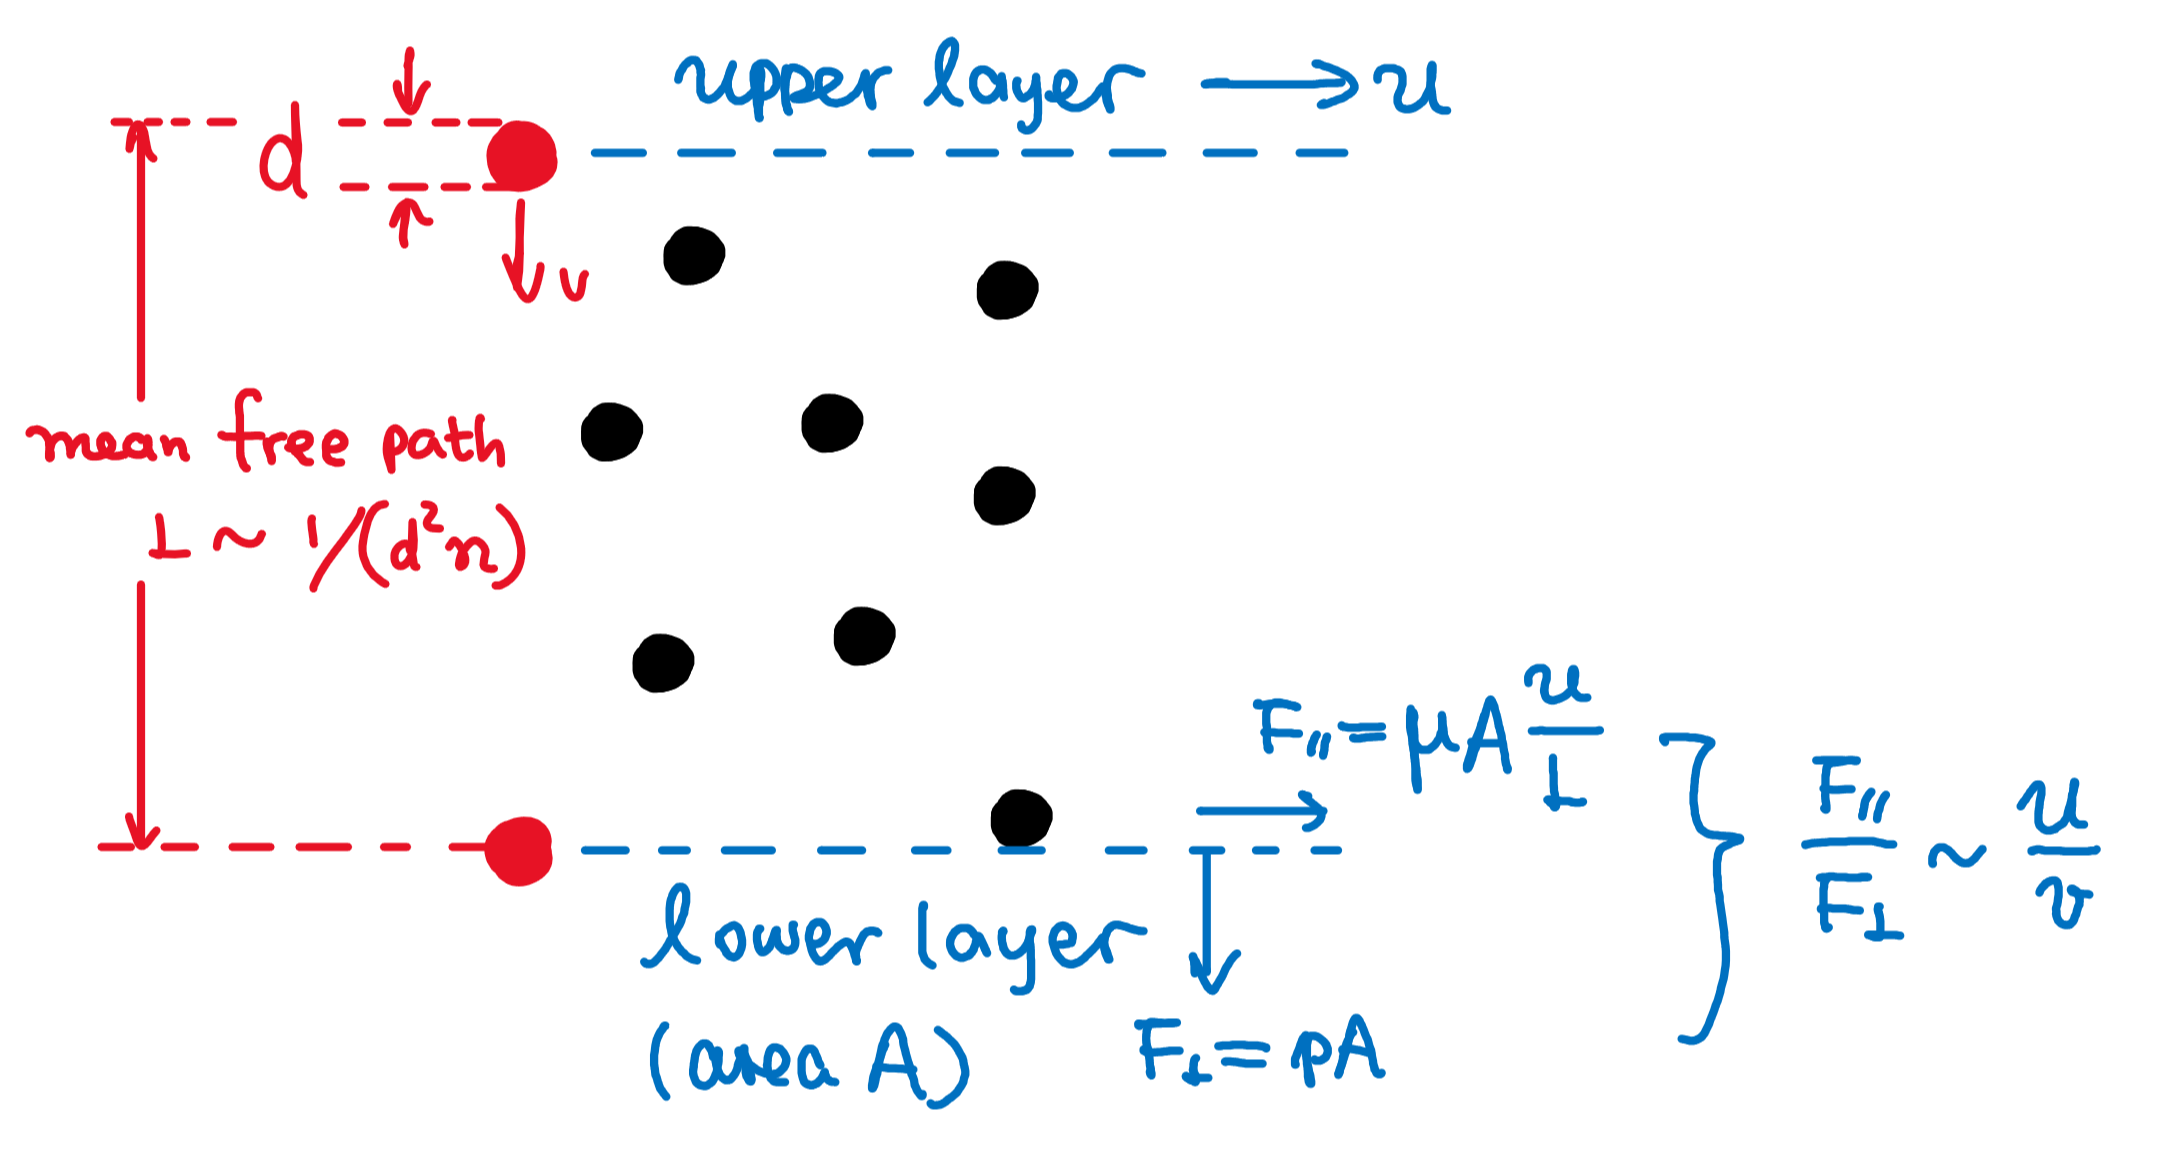
\includegraphics[width=0.7\textwidth]{viscosity}
    \end{center} 

    The viscosity $\mu$ of the gas is defined as
    \begin{align}
        F_{\parallel} = \mu A u / y~,
    \end{align}
    where $A$ is the area of each layer and $y$ is the distance between layers. And $u$ is the non-random part of the motion speed between layers. The viscosity of air is $\mu \sim 10^{-5} \mbox{kg} / \mbox{m} / \mbox{s}$.
    
    As shown in the above figure, we consider two layers of gas, separated by $y=L$. Then on average, the force is passed on from the upper layer to the lower layer by order-one collision. We expect that the force normal to the lower layer $F_\perp = p A$ can be related to $F_{\parallel}$ by
    \begin{align}
        \frac{F_\parallel}{F_\perp} \sim \frac{u}{v}~, 
    \end{align}
    since they come from the same collisions (having the same time duration of collision $\Delta t$ in the impulse).

    Putting the above equations together, the mean free path of air is thus
    \begin{align}
        L \sim \frac{\mu v}{p} \sim 10^{-7} \mbox{m}~.
    \end{align}
}

Amazingly, without being able to see a single atom (at that time), one can infer the speed and mean free path of atoms! Further, can we also determine the size of atoms?

\textbox{The size of an atom\index{atom:size}}{
    Loschmidt (1865) determined the size of atoms with a very simple observation (based on the above mean free path). When gas liquify at low temperature, its volume condenses by a factor of about 1000 (and when liquid solidify the volume does not change much). The number density of liquid and solid $\tilde n$ can be estimated by
    \begin{align}
        \tilde n \sim d^{-3} \sim 1000 n \sim 1000 d^{-2} L^{-1}~.
    \end{align} 
    Here it is assumed that in liquid and solid the atoms are close to each other. Thus, the size of an atom is estimated by
    \begin{align}
        d \sim 10^{-3} L \sim 10^{-10} \mbox{m}~.
    \end{align}
}

By the end of the 19th century, the atomic theory has gained great success. As Sir William Thomson commented in 1889, the atomic theory is
% Sir William Thomson, Popular Lectures and Addresses, Vol. I., London, 1889, p. 148.
\begin{quote}
    ... founded respectively on the undulatory theory of
    light, on the phenomena of contact electricity, on capillary
    attraction, and on the kinetic theory of gases, agree in 
    showing that the atoms or molecules of ordinary matter must be
    something like the l/10,000,000th, or from the l/10,000,000th
    to the l/100,000,000th, of a centimeter in diameter.
\end{quote}

However, the atomic theory still receive some criticism (for example, by Mach) since no one has actually seen an atom. Is the atomic theory just an ``effective'' theory to explain experiments, or are atoms indeed the building blocks of our \emph{real} world? 

\textbox{(Optional) Brownian motion\index{Brownian motion}}{
    In
    \marginnote{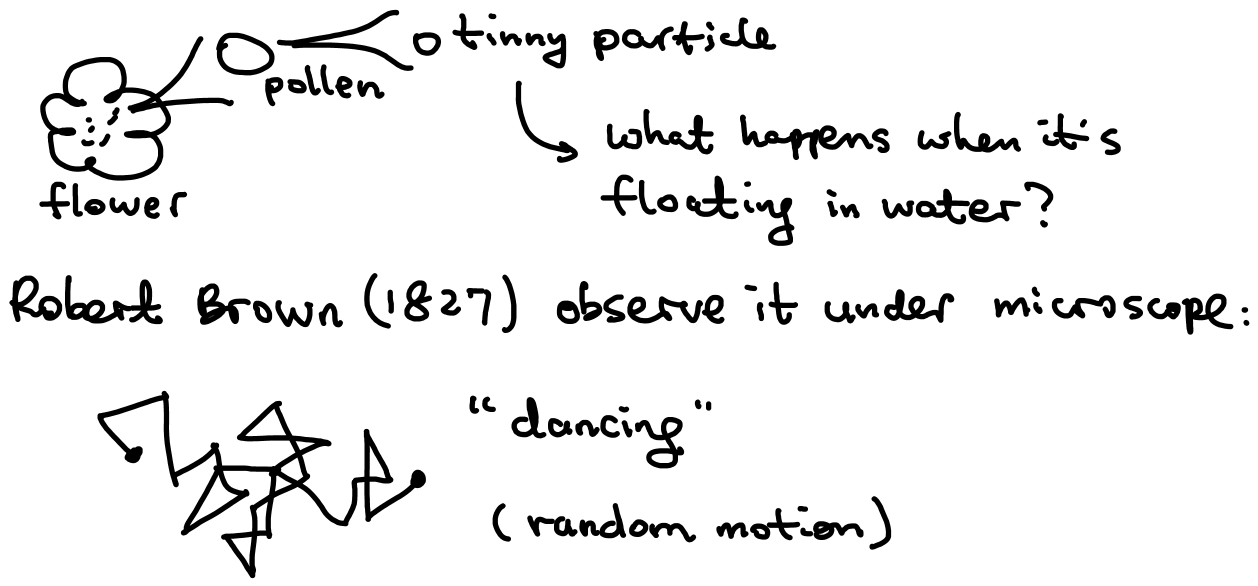
\includegraphics[width=0.4\textwidth]{brownian}} 
    1827, Robert Brown notices that tinny particles from pollen ``dance'' in the water. Einstein in 1905 explained the dancing particles by the motion of molecules -- we actually see their direct effects. Here we use Langevin's stochastic differential equations (1908) to describe Einstein's idea.

    The particle from pollen is constantly kicked by water molecules. The speed of the particle satisfy the following Langevin equation\index{Langevin equation}
    \begin{align}
        M \frac{dv}{dt} = -\lambda v + f(t)~,    \label{eq:lang}
    \end{align}
    where
    \titem{
        \item The parameter $M$ is the mass of the particle.
        \item The parameter $\lambda$ describe a friction force, i.e. dissipation in water. This dissipation can be measured by, say, measuring the terminal velocity of a heavy ball in deep water.
        \item The function $f(t)$ is force from random kick on the particle by molecules. The random force can be modeled by white noise: 
        \begin{align}
          \label{eq:f_rand}
          \langle f(t) \rangle = 0~, \qquad 
          \langle f(t) f(t') \rangle = \Lambda \delta(t-t')~.
        \end{align}
        Similarly to the notation in quantum mechanics, here $\langle \cdots \rangle$ means taking average. 
        \marginnote{To very good approximation, the random kicks are independent of each other. Thus the kicks at different time has no correlation between each other. But at the same time, the ``same'' kick has self correlation. This is why $\langle f(t) f(t') \rangle$ is propotional to $\delta(t-t')$. The parameter $\Lambda$ characterize how fast the particle fluctuates.}
        $\Lambda$ can be measured as follows: given a set of particles initially at coincide positions, due to the fluctuation, the particles diffuse and one can obtain $\Lambda$ by the speed of diffusion for the set of particles.
    }
    The Langevin equation \eqref{eq:lang} can be solved by ``variation of constants'' method:
    \begin{align}
        \label{eq:sol_lang}
        v(t) = v_0 e^{-\frac{\lambda}{M} t}
        + \frac{1}{M}  \int_0^{t} dt_1 f(t_1) e^{-\frac{\lambda}{M}(t-t_1)} ~.      
    \end{align} 
    Thus,
    \begin{align}
        \langle v(t) \rangle = \langle v_0 \rangle e^{-\frac{\lambda}{M} t}~.
    \end{align}
    \begin{align}
        \label{eq:lang_v2}
        \langle v^2(t) \rangle & = \langle v_0^2 \rangle e^{-2\frac{\lambda}{M} t}
        + \frac{1}{M^2} \int_0^t dt_1 \int_0^t dt_2 
        e^{-\frac{\lambda}{M}(t-t_1)} e^{-\frac{\lambda}{M}(t-t_2)}
        \langle f(t_1) f(t_2) \rangle
        \nonumber\\ &
        = \langle v_0^2 \rangle e^{-2\frac{\lambda}{M} t}
        + \frac{\Lambda}{2M\lambda} \left ( 1-e^{-2\frac{\lambda}{M} t} \right )~. 
    \end{align}
    After a long time $t$, the exponentially suppressed terms (memory about the initial condition) dies out. As a result, we have vanishing $\langle v(t) \rangle$, and \marginnote{Note that $\frac{1}{2}  M\langle v^2(t) \rangle = \frac{1}{2} k_B T$. Thus this is a direct measurement of the Boltzmann's constant $k_B$. In 1908, such a measurement is made by Perrin.}
    \begin{align}
    \label{eq:lang_v2_infty}
        \frac{1}{2}  M\langle v^2(t) \rangle & = \frac{\Lambda}{4\lambda}~. 
    \end{align}
    We have thus computed the average kinetic energy of the particle. Note that this energy should be statistically the same as the kinetic energy of a molecule in the water. Because otherwise the particle will pass energy to water molecule and lose energy (equipartition theorem). Compared to total internal energy per unit volume, we know how many atoms there are and thus their size. 
}

\needspace{0.3\textheight}
\mtextbox{Distance ladders}{
    We encountered three methods of measuring the size of an atom. In each case, a distance ladder is built from human accessible scales to a microscopic scale.
    \mtitem{
        \item Oil film: through oil-alcohol solution.
        \item Kinetic theory: through three large or small numbers: air pressure, viscosity and condensation rate from gas to liquid.
        \item Brownian motion: through motion of tinny particle from pollen.
    }
    \tcblower
    Distance ladder is an important technique for accessing distances that we are not yet able to reach. This is true also for larger distances, for example the measurement of distance in astronomy and cosmology.
}
\textbox{(Optional) Fluctuation and dissipation: another equivalence from Einstein\index{fluctuation-dissipation theorem}}{
    The interpretation of Brownian motion is another Einstein-style discovery. Let's take a closer look at the two measurable quantities involved in Brownian motion:  $\Lambda$ denote the strength of fluctuation; and $\lambda$ denote the rate of dissipation. They are at the first sight unrelated. But Einstein noted that they are of the same origin.

    Why there is dissipation? Macroscopically it is from viscosity or friction. While microscopically it is from the fact that, imagine that you are the particle, once you run forward, there are more molecules hitting your face than your back, with a greater speed. Thus the random knocks tends to block your motion. This related dissipation to fluctuation. 

    This observation can be generalized to a fluctuation-dissipation theorem in statistical physics. It has a wide range of applications. For example, the thermal noise (Johnson-Nyquist noise) in a resistor is related to its resistance by the same observation. The discussion can even (sloppily) be applied to social science -- a creative society (more fluctuations) is often lack of executive ability (more dissipation) and it's a challenge to keep both.
}

\section{The Hydrogen Atom} \label{sec:atom-hydrogen}

Now that we have understood that matter is made of atoms, let us study the nature of atoms. We start from the simplest atom: the hydrogen atom.

\subsection{Aspects of observations}

Since Newton, lots of scientists studied the spectrum of light. Since matter is made by atoms, light emitted/absorbed by matter is also (usually) emitted/absorbed by atoms as well. Can we learn about the nature of atoms from the study of 
\marginnote{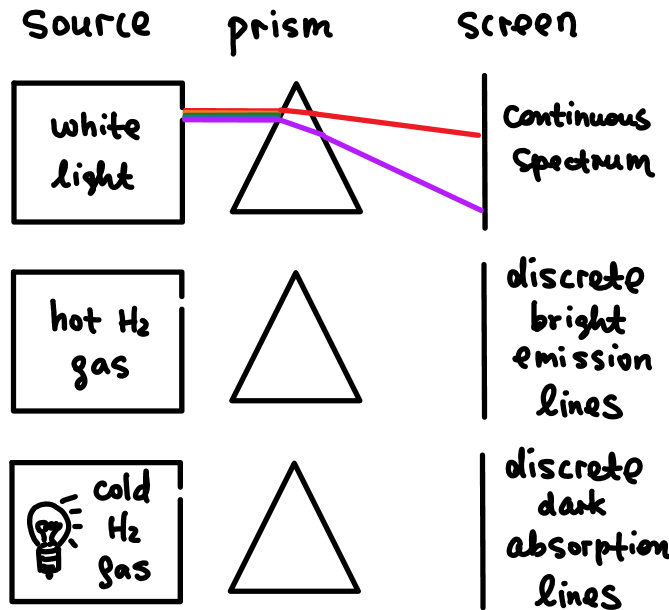
\includegraphics[width=0.35\textwidth]{hlines}}
light spectrum?

% reference: http://web.mit.edu/spectroscopy/history/history-classical.html
\textbox{Developments in spectroscopy\index{atom:spectroscopy}}{
    \titem{
        \item 1666, Newton: used prism to split the sunlight into a spectrum.
        \item 1814, Fraunhofer: dark lines in the sun spectrum.
        \item 1817-1823, Fraunhofer: spectra from the moon, Venus and Mars has some dark lines at the same position of the sun spectrum, and also some new lines.
        \item 1826, Herschel and Talbot: emission spectrum, different elements have different spectra (spectra to elements like fingerprints to human).
        \item 1832, Brewster: Dark lines in the sun spectrum are absorption lines by its atmosphere.
        \item 1859, Kirchhoff: Emission and absorption lines have the same position.
        \item 1860-1861, Kirchhoff and Bunsen: Discovered elements (cesium and rubidium) by their spectra (like catching criminals by fingerprints).
        \item 1885, Balmer: found a formula for the Hydrogen spectrum for visiable light frequencies, see the
        \marginnote{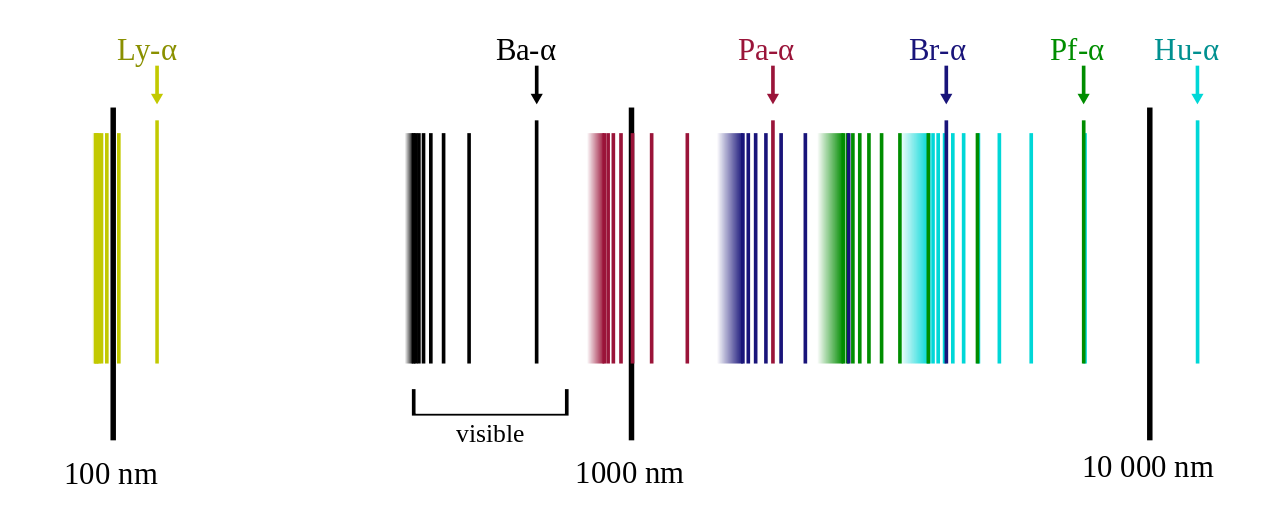
\includegraphics[width=0.4\textwidth]{hlines_wp}\newline The spectral lines of Hydrogen atom. Figure from Wikipedia.}
        margin figure. In the below equation, $R_H$ is a constant.
        \begin{align}
          \label{eq:Blamer_line}
          \frac{1}{\lambda} = R_H \left ( \frac{1}{4} - \frac{1}{n^2}  \right )~,
          \quad n=3,4,5,\ldots
        \end{align}
        \item 1888, Rydberg: proposed a general formula for Hydrogen
        \begin{align}
          \label{eq:Rydberg_line}
          \frac{1}{\lambda} = R_H \left ( \frac{1}{m^2} - \frac{1}{n^2}  \right )~,
          \quad n=m+1, m+2,\ldots
        \end{align}
        \item 1906, Lyman: ultraviolet bands of Hydrogen spectrum ($m=1$ of \eqref{eq:Rydberg_line}).
        \item 1908, Paschen: infrared bands of Hydrogen spectrum ($m=3$ of \eqref{eq:Rydberg_line}).
    }
}

How to understand such spectra of elements? A simple equation such as \eqref{eq:Rydberg_line} deserves a theory. We need to understand in details how atom interacts with light -- knowing the inner structure of atoms should help. Thus, let us review briefly another line of research in the history -- the subatomic structure.

\textbox{The discovery of the subatomic structure\index{subatomic structure}}{
    It was shocking to know that atoms are not actually the fundamental building blocks of matter. They are made of even smaller particles.
    \titem{
        \item 1897, Thomson: Discovery of electron.
        \item 1899, Rutherford: Discovery of $\alpha$ particle (Helium nuclei).
        \item 1904, Thomson: the plum pudding model of atom.
        \item 1909, Geiger, Marsden, Rutherford, $\alpha$ particle scattering.
        \item 1911, Rutherford: nuclei-electrons model, like sun-planets that electron runs in orbits around the nuclei. The nuclei radius is about $10^{-5}$ of an atom.    
    }
    \tcblower 
    Rutherford's atom model has a serious problem: Electron must have acceleration when moving within the atom volume. However, acceleration of charge implies E\&M radiation. The electron should then lose energy and fall onto the nuclei. 

    How to stabilize Rutherford's atom and save the world?
}

Now, both the studies of spectroscopy and subatomic structure have evolved to the 1910s. At that time physicists start to appreciate the need of quantum mechanics. Would quantum mechanics play a role to solve the problem of subatomic structure, and/or explain the atom spectrum?


\subsection{Bohr's Model of the Hydrogen Atom}

\textbox{Bohr's model\index{Bohr's atomic model}}{
    In 1913, Bohr brought together 3 aspects of physics, to build up his atomic model:
    \tenum{
        \item Atomic spectroscopy: There are different frequencies of light:
        \begin{align}
          \label{eq:rydberg_nu}
          \nu^{(n_2, n_1)} = \frac{c}{\lambda^{(n_2, n_1)}} = c R_H 
          \left ( \frac{1}{n_2^2} - \frac{1}{n_1^2}   \right )~.
        \end{align}
        \item Quantum nature of photon: Frequency of light originates from the energy of photon: $E_\gamma^{(n_2, n_1)}=h\nu^{(n_2, n_1)}$.
        \item Subatomic structure: In a hydrogen atom, the electron can be on different orbits. Classically, those orbits correspond to different energy of the electron. First note force:
        \begin{align}
          \label{eq:orbit_bohr_electron}
          F = \frac{mv^2}{r} = \frac{1}{4\pi\epsilon_0}\frac{e^2}{r^2}
          \quad\Rightarrow\quad mv^2 = \frac{1}{4\pi\epsilon_0}\frac{e^2}{r}
        \end{align}
        Thus the energy of the electron is
        \begin{align}
          \label{eq:energy_bohr_electron}
          E_e = \frac{1}{2} mv^2 + V(r) = - \frac{1}{2} m v^2~.
        \end{align}  
    }
    \tcblower
    Now let's put them together. The frequency of the electron on such an orbital is $\nu_e = v / (2\pi r)$. It is natural to expect that for an electron to move from infinity at rest to a orbital, the frequency of photons emitted is related to this frequency. 
    Bohr suggests that
    \marginnote{Here the factor of 2 is a guess, probably as a naive average between $\nu_e$ and 0, which is the inital frequency for an electron at infinity. Don't worry, we will soon get rid of Bohr's atom. The Schr\"odinger equation can compute everything clearly.}
        \begin{align}
            \nu = \frac{\nu_e}{2} = \frac{v}{4\pi r}~.  
        \end{align}
    As the emission is quantized, we have
    \begin{align} \label{eq:emvr}
        |E_e| = n h \nu \quad\Rightarrow\quad m v r = \frac{nh}{2\pi}~,
    \end{align}
    where $n$ is an integer. Using \eqref{eq:orbit_bohr_electron} to cancel $r$, \eqref{eq:emvr} can be written as
    \begin{align}
        v = \frac{e^2}{2n\epsilon_0 h} \quad\Rightarrow\quad
        E_e(n) = -\frac{m e^4}{8\epsilon_0^2h^2} \times \frac{1}{n^2}~. 
    \end{align}
    This indeed derives Eq. \eqref{eq:rydberg_nu}:
    \begin{align}
    \nu^{(n_2, n_1)} = c R_H 
    \left ( \frac{1}{n_2^2} - \frac{1}{n_1^2}   \right )~,
    \qquad
    R_H = \frac{me^4}{8\epsilon_0^2h^3 c}~. 
    \end{align}
}

\textbox{Relation to de Broglie's matter wave}{
    The quantization condition \eqref{eq:emvr} can be understood in an intuitive way: the equation can be rewritten as
    \begin{align}
        \frac{p}{\hbar} = \frac{n}{r}~,  
    \end{align}
    where the momentum of the electron is $p=mv$, and $\hbar = h / (2\pi)$.

    Requiring
    \marginnote{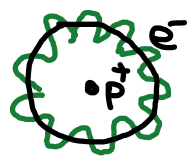
\includegraphics[width=0.15\textwidth]{bohr_atom}}
    the electron on the orbital being standing wave (satisfying periodic boundary condition), we note that $n/r = k$ is the wave number. And thus \eqref{eq:emvr} is nothing but the de Broglie's matter wave $p=\hbar k$ (which is proposed in 1924, historically much later than Bohr's atom).
}

Although Bohr's theory of atom is successful in explaining the Hydrogen spectrum to certain accuracy, it is unable to explain the fine structure of Hydrogen, or the spectra of multi-electron atoms.

Now we know that those failures of Bohr's model is because of the semi-classical nature of Bohr's model. The electron's position and momentum satisfies the uncertainty principle. Thus there is no classical orbits. Those difficulties are indeed gone after the full quantum mechanics is taken into account.


\subsection{(Optional) The Schr\"odinger Equation of the Hydrogen Atom}
\label{sec:schrodinger-atom}

In this subsection, we present the technical details for solving the Schr\"odinger equation, as optional material. We will scratch the procedure without presenting the full details here.


\textbox{The 3-dimensional Schr\"odinger equation}{
    In 3 dimensions, the stationary state Schr\"odinger equation is\marginnote{In this section, we denote the mass of the quantum particle by $M$ instead of $m$ because traditionally $m$ is used to label the magnetic quantum number (see definition below).}
\begin{align}
  \label{eq:Schrodinger3d}
  \left [ 
    -\frac{\hbar^2}{2M} 
        (\partial_x^2 + \partial_y^2 + \partial_z^2)
    + V
  \right ] \psi = E \psi ~, \qquad   V \equiv V(r) \propto \frac{1}{r} ~,
\end{align}
or equivalently,
\begin{align}
  \label{eq:Schrodinger3d1}
  (\partial_x^2 + \partial_y^2 + \partial_z^2) \psi
  + \frac{2M}{\hbar^2} (E-V) \psi = 0 ~.
\end{align}
Now we get a Schr\"odinger equation with derivatives in all $x,y,z$ directions. A differential equation with different types of partial derivatives is known as a partial differential equation. How to solve it?
}

\textbox{Spherical coordinates}{
    To solve this equation, one first note that the potential has spherical symmetry. Thus spherical coordinates fits better to solve the equation. In spherical coordinates, the differential operators of the above equation is rewritten into
\begin{align}
  \label{eq:Schrodinger3dsd}
  (\partial_x^2 + \partial_y^2 + \partial_z^2) \psi
  = \frac{1}{r^2} \partial_r (r^2\partial_r\psi)
  + \frac{1}{r^2\sin\theta} \partial_\theta (\sin\theta\partial_\theta\psi)
  + \frac{1}{r^2\sin^2\theta} \partial_\phi^2\psi ~.
\end{align}
}

\mtextbox{Spherical harmonics}{
    In fact, we can pack a good part of the procedure here into known math -- the solution of the angular directions can be directly written as the spherical harmonics: $\Theta(\theta)\Phi(\phi) \propto Y_{\ell m}(\theta, \phi)$. The spherical harmonics $Y_{\ell m}(\theta, \phi)$ is already well studied in the 18-19 century for studying classical wave equations on a sphere. But here we still use $\Theta(\theta)\Phi(\phi)$ since:
    \mtitem{
        \item You may not be familiar to $Y_{\ell m}(\theta, \phi)$.
        \item We'd like to open the black box of math to see what actually happens here.
    }
}
\textbox{Separation of variables}{
    Now we use a smart trick -- separation of variables. This is a powerful method in solving a class of partial differential equations. We assume that the solution takes the form
\begin{align}
  \label{eq:separation_of_vars}
  \psi(r, \theta, \phi) = R(r)\Theta(\theta)\Phi(\phi)~.
\end{align}
The Schr\"odinger equation now can be written as
\begin{align} \label{eq:schrtp}
  & \frac{1}{R} \partial_r \left ( r^2 \partial_r R \right )
  + r^2 \frac{2M}{\hbar^2} [E-V(r)]
\nonumber\\
  +& \frac{1}{\Theta \sin\theta} \partial_\theta 
        \left ( \sin\theta \partial_\theta \Theta \right )
  + \frac{1}{\Phi \sin^2\theta} \partial_\phi^2 \Phi  = 0~.
\end{align}
This equation has interesting structure: the first line of the equation only depends on $r$ and the second line of the equation does not depend on $r$. As a result, the first line cannot depend on $r$ either and thus must be a constant:
\begin{align}\label{eq:schr}
  \frac{1}{R} \partial_r \left ( r^2 \partial_r R \right )
  + r^2 \frac{2M}{\hbar^2} [E-V(r)] = \ell (\ell + 1)~.
\end{align}
With this observation, the second line of \eqref{eq:schrtp} can be written as
\begin{align}
  & \frac{\sin\theta}{\Theta} \partial_\theta 
        \left ( \sin\theta \partial_\theta \Theta \right )
  + \ell (\ell + 1) \sin^2\theta
  \nonumber\\
  + & \frac{1}{\Phi}\partial_\phi^2 \Phi = 0~. 
\end{align}
Again, this new equation has similar structure: The first line depends only on $\theta$ and the second line does not depend on $\theta$. Thus both of them must be constants. We thus have
\begin{align}\label{eq:scht}
  \frac{\sin\theta}{\Theta} \partial_\theta 
        \left ( \sin\theta \partial_\theta \Theta \right )
  + \ell (\ell + 1) \sin^2 \theta = m^2~.
\end{align}
\begin{align}\label{eq:schp}
  \partial^2_\phi \Phi + m^2 \Phi = 0~.
\end{align}
The partial differential equation, outstandingly, factorize into three ordinary differential equations: Eqs.~\eqref{eq:schr}, \eqref{eq:scht} and \eqref{eq:schp}. Ordinary differential equations are much easier to deal with. Nevertheless, we are not going to fully solve those equations for you. We are going to solve \eqref{eq:schp} only as it is a familiar wave equation. We give the physical result of \eqref{eq:schr} and \eqref{eq:scht} without diving into full details.
}

\textbox{The $\Phi$ equation: the magnetic quantum number $m$ with $L_z = m \hbar$}{
    It is easy to check that Eq.~\eqref{eq:schp} has solution\marginnote{In general, we have $\Phi = c e^{im\phi}$ with a constant $c$. This constant is not relevant and is omitted. Also, there is another set of solution $\Phi = e^{-im\phi}$. That solution corresponds to $m\rightarrow -m$.}
\begin{align}
  \Phi = e^{im\phi}~.
\end{align}
They are just left and right moving waves in the angular direction (w.r.t. the $z$-axis). Physically, $m$ is related to the angular momentum. The angular momentum in quantum mechanics is $\mathbf{L} = \mathbf{r} \times \mathbf{p} = -i\hbar (r\times \nabla)$. One can derive that $L_z = -i\hbar \partial_\phi$ in spherical coordinates. As a result, $L_z = m\hbar$.

Note that the wave has periodic boundary condition 
\marginnote{The math structure here is similar to Bohr's semi-clssical atom. However, the physics is different. We did not confine the electron to move along the $\phi$-direction only. Rather, now we are just calculating the wave function on the $\phi$-direction. The electron has probability to appear anywhere instead only on the orbital.}
(recall the continuity requirements of the wave function):
\begin{align}
  \Phi |_{\phi=0} = \Phi |_{\phi} = 2\pi~,
  \qquad
  \partial_\phi \Phi |_{\phi=0} = \partial_\phi \Phi |_{\phi = 2\pi}~.  
\end{align}
To satisfy those conditions, $m$ must be integers and is known as the magnetic quantum number.\index{magnetic quantum number} 
}

\textbox{The $\Theta$ equation: the azimuthal quantum number $\ell$.}{
    Now we look at the equation \eqref{eq:scht}. We shall not solve the equation here (you will learn the solution in a proper QM class). But recall our experience of the $\phi$ direction: There are two similarities:
\tenum{
  \item Note that $\theta$ is also rotation so should be related to some sort of angular momentum. As a result, $\ell$ should be related to some sort of angular momentum. As we will see soon, the total momentum of the wave function is
  \begin{align}
    L^2 = \ell (\ell + 1)\hbar^2~.
  \end{align}
  \item For the solution $\Theta(\theta)$ to be regular at $\theta=\pi$, it turns out that $\ell$ should take integer values only. It turns out\marginnote{As we have argued that $m$ is related to the angular momentum in the $z$-direction and $\ell$ is related to the total angular momentum, it is natural to understand that $m$ should not exceed $\ell$.} that $\ell$ (known as the azimuthal quantum number\index{azimuthal quantum number}) can only take integer values starting from $m$: $\ell = m, m+1, \ldots$ We can rearrange this requirement into
  \begin{align}
    \ell = 0, 1, 2,3,4,5,6, \ldots~,
  \end{align}
  and those orbitals are known as s, p, d, f, g, h, i, $\ldots$ in chemistry. For a given $\ell$, $m$ is restricted to be
  \begin{align}
    m = 0, \pm 1, \ldots, \pm \ell~.
  \end{align}
}
}

\needspace{0.3\textwidth}
\mtextbox{The total angular momentum}{
    Adding a factor $\frac{\hbar^2}{2Mr^2} \ell (\ell + 1)$ to the potential looks familiar. In classical mechanics, when reducing a 3d central-force problem into 1d, the additional term added into the effective potential is $\frac{L^2}{2Mr^2}$, where $L$ is the total angular momentum of the electron. Comparing it to \eqref{eq:schr-alt}, we conclude that the angular momentum of the system is $L^2 = \ell (\ell + 1)\hbar^2$.
}
\textbox{The $R$ equation: The principal quantum number $n$\index{principal quantum number}}{
    Finally, we will get some feeling from Eq.~\eqref{eq:schr}, again without fully solving it. We can rewrite Eq.~\eqref{eq:schr} as
\begin{align}\label{eq:schr-alt}
  \frac{1}{R} \partial_r \left ( r^2 \partial_r R \right )
  + r^2 \frac{2M}{\hbar^2} \left[
    \left(E - \frac{\hbar^2}{2Mr^2} \ell (\ell + 1)\right)-V(r)
  \right] = 0~.
\end{align}
This is similar to a stationary Schr\"odinger equation, with reduced energy. The reduction of energy is because we are interested in a reduced one-dimensional problem and thus must deduct the energy coming from rotation. 

This is a bound state problem. Thus the energy spectrum is discrete. After solving \eqref{eq:schr-alt} (which is technical and we skip the details here), one eventually finds
\begin{align}
  E = \frac{E_1}{n^2}~, \qquad 
  E_1 \equiv - \frac{m e^4}{32\pi^2 \epsilon_0^2 \hbar^2}~.
\end{align}
Here $n$ is an integer with $n=\ell + 1, \ell + 2, \ldots$. This is the result of quantized energy levels that Bohr obtained.

It is intuitive that the starting integer for $n$ must be bounded by $\ell$ because the larger $\ell$, the larger energy from angular momentum, to be deducted from $E$. One can again rewrite the requirements for $n, \ell, m$ as:
\begin{align}
  n=1,2,\ldots~, \quad
  \ell = 0, 1, \ldots, n-1~, \quad
  m = 0, \pm 1, \pm 2, \ldots \pm \ell~.
\end{align}
}

\subsection{Properties of the Hydrogen Atom}

As the previous subsection is optional and you may like to skip that, here we summarize the properties of the atom, and discuss their physical consequences.

\textbox{Number of possible atomic states}{
    Given $n, \ell, m$, we can count the number of possible states. This is of crucial importance in chemistry. For the counting, we first note two things about electrons:
\begin{itemize}
  \item Electrons are fermions and thus they cannot be in the same state.
  \item For each given set of $n, \ell, m$, there are two electron states. This is because electron has spin $m_e = \pm 1/2$, namely spin up and spin down.
\end{itemize}
We can now count the number of possible atomic states. For example, for $n=1$, we must have $\ell =0, m=0$ thus two states (because of spin of electron). For $n=2$, we have
\begin{align}
  \begin{cases}
    \ell = 0, m=0, m_e = \pm 1/2, &\quad\mbox{2 states}\\
    \ell = 1, m=0, m_e = \pm 1/2, &\quad\mbox{2 states}\\
    \ell = 1, m=\pm 1, m_e = \pm 1/2 &\quad\mbox{4 states},
  \end{cases}
\end{align}
thus in total 8 states. In general, for given $n$, there are $2n^2$ states.

The states with the same $n$ is said to be in the same shell; the states with the same $n$ and $\ell$ is said to be in the same orbital.\index{shell}\index{orbital}
}

\textbox{The electron cloud\index{electron cloud}}{
    Now 
    \marginnote{
    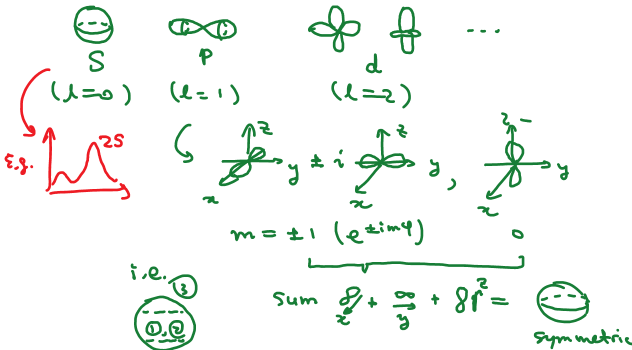
\includegraphics[width=0.4\textwidth]{e_cloud}}
    with the wave function $\Psi(r, \theta, \phi)$, the property of the electron is expressed in terms of the probability density amplitude (such a distribution is known as the electron cloud). This is different from classical orbitals. Nevertheless, we can still use the term ``orbitals'' to denote the states with different $n$, $\ell$ and $m$. Some of the states are illustrated in the side figure.

    For each $n$, the s, p, d, $\ldots$ orbitals has the features illustrated below. One notes that the s orbital has greater probability density at both small $r$ and large $r$ than p and d.

    Pay attention to the oscillations in the probability distribution. 
    \marginnote{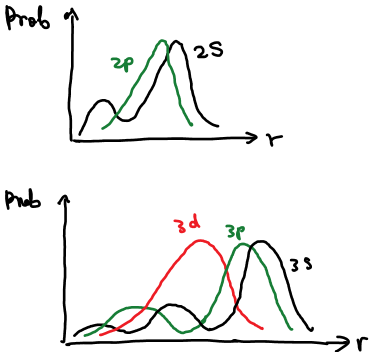
\includegraphics[width=0.35\textwidth]{spd2}}
    Although we have not calculated them explicitly here, they are understandable from our experience in the bound states in an infinitely deep potential well.
}
\textbox{Transitions and selection rules\index{selection rules}}{
    Now that we know the Hydrogen atom (in general all atoms) can be in stationary states with definite energy. There can be transition between those states. Namely, an atom can emit a photon and become a lower energy state; or absorb a photon and become a higher energy state. From energy conservation, the frequency of the photon is
\begin{align}
  \nu = \frac{E_{n'}-E_n}{h}~, 
\end{align}
where the two states $E_{n'}$ and $E_n$ must satisfy $\Delta \ell = \pm 1$, $\Delta m_\ell = 0, \pm 1$. This is because a photon has spin 1.
}

\section{The Periodic Table} \label{sec:atom-multi}

Now
\marginnote{For multiple electron atoms -- even for helium, the Schr\"odinger equation cannot be solved analytically. One may either try to solve it numerically or study the qualitative features from our experience of the hydrogen atom.}
we are interested in elements other than Hydrogen. What happens for an atom with a nuclei with $Z$ positive charges? 

\textbox{Qualitative differences for many-electron atoms}{
    \titem{
        \item Pauli's exclusion principle: If one orbital is filled, the other electrons in the atom must be put in other orbitals.
        \item Screening and other electron interactions: 
        \marginnote{In general electron interactions are very complicated. For example, in some sense the Helium electron interaction problem is a quantized 3-body problem. Fortunately, the ``screening'' point of view can provide us some intuitions and is sometimes a good approximation.}
        Classically, the inner electrons screen the charge of the nuclei when we consider the motion of outer electrons. In quantum mechanics, there is no absolute inner/outer electrons. But the spatial distribution of electrons needs to be considered in the screening effect. As a result, in a hydrogen atom for the same $n$, s,p,d,f,... orbitals has the same energy. But for multiple electron atoms, for the same $n$, $E_s<E_p<E_d<E_f$ because higher angular momentum means (on average) farther from the nuclei and thus more screening.
    }
}

To see how these features affect the electron configurations of elements, especial the outermost occupied shell (called the valence shell which is mostly responsible for its chemical properties), we list some elements and how the electrons are configures in them. We will only discuss the ground states.

\textbox{Electron configurations of some elements}{
    \titem{
        \item Hydrogen: 
        \marginnote{Hydrogen (H, $Z=1$) \mnewline
            \begin{MOdiagram}[style=square]
                \AO{s}[label={1s}]{0;up}
            \end{MOdiagram}
        }
        For the ground state of hydrogen, the electron is in $n=0$ state. There is only a s-orbital ($\ell = 0$). The electron has an ionization energy (the minimal energy to remove an electron to infinity) of 13.6 eV.
        \item Helium:
        \marginnote{\newline Helium (He, $Z=2$) \mnewline
            \begin{MOdiagram}[style=square]
                \AO{s}[label={1s}]{0}
            \end{MOdiagram}
        }   
        Naively, the ionization energy of helium would be $Z^2 \times 13.6 \mbox{eV}= 54.4\mbox{eV}$. However, actually its ionization energy is 24.5 eV. This is because of screening. In fact, after taking away the first electron of helium, we indeed need about $54.4\mbox{eV}$ to take its second electron away (the second ionization energy).

        As helium has full filled its valence shell, it is hard to offer or accept electrons to other atoms to form chemical bound. Thus, its chemical property is very stable.
        \item Lithium:
        \marginnote{Lithium (Li, $Z=3$) \mnewline
            \begin{MOdiagram}[style=square]
                \AO{s}[label={2s}]{0;up}
                \AO(30pt){p}[label={2p}]{0.2;}
            \end{MOdiagram}
        }
        With 3 electrons, one electron has to go to the $n=2$ shell. Will the electron be filled in the 2s ($\ell=0$) orbital or the 2p ($\ell=1$) orbital? Due to screening, the s-orbital has lower energy thus the electron is filled in the s-orbital. The ionization energy of lithium is 5.45 eV. It's very easy to lose such an electron and thus lithium has active chemical property.
        
        \item From beryllium to Argon, we fill additional electrons as discussed above: 2s, 2p, 3s, 3p.
        
        \item Potassium:
        \marginnote{Potassium (K, $Z=19$) \mnewline
            \begin{MOdiagram}[style=square]
                \AO{p}[label={3d}]{0;}
                \AO(60pt){s}[label={3d}]{0;}
                \AO(80pt){s}[label={3d}]{0;}
                \AO(110pt){s}[label={4s}]{-0.2;up}
            \end{MOdiagram}
        }
        naively we would have proceeded to fill 3d after 3p. However, as the 3d orbital has too large angular momentum, it actually have slightly greater energy than 4s. As a result, for potassium, 4s is filled first.
    }
}

\needspace{0.1\textwidth}
Hopefully, the above discussion provides some physical understanding for the periodic table.\index{periodic table}
\marginnote{\begin{center}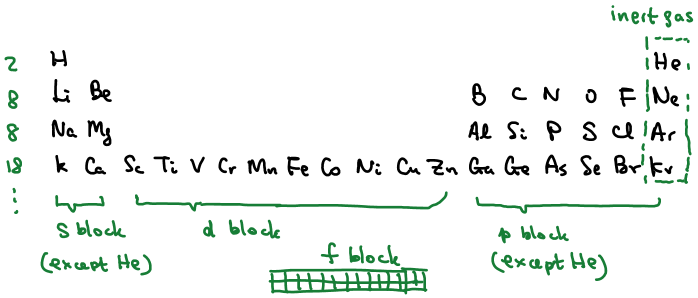
\includegraphics[width=0.35\textwidth]{ptab}\end{center}}

\section{Epilogue: Summary and What's Next}

\textbox{Further reading about the content}{
    \titem{
        \item For the size of the atom, more details can be found in \href{http://www.informationphilosopher.com/solutions/scientists/maxwell/illustrations_dynamical_theory_gases_1.pdf}{Maxwell} and \href{https://www.chemteam.info/Chem-History/Loschmidt-1865.html}{Loschmidt}'s original works. Maxwell's paper contains lots of technical calculations while Loschmidt's paper is very simple to understand.
        \item Although Bohr's atomic model is exceeded by the Schr\"odinger equation approach, if you are interested in more historical details, you can read \href{http://hermes.ffn.ub.es/luisnavarro/nuevo_maletin/Bohr_1913.pdf}{Bohr's origonal paper}.
        \item For the Schr\"odinger equation and the periodic table, more details can be found at the \href{http://www.feynmanlectures.caltech.edu/III_19.html}{Feynman Lectures III Chapter 19}. For even more details related to chemistry, you may like to read a book on physical chemistry, for example \href{https://www.amazon.com/Physical-Chemistry-Robert-J-Silbey/dp/047121504X}{Physical Chemistry by Silbey, Alberty and Bawendi}.
    }
}

\textbox{What happens next?}{
    The quantum part of the content here will be studied in more details in quantum mechanics and physical chemistry.

    The atomic and sub-atomic structure of matter is just a starting point of exploring the inner matter structures, instead of an end. The research on particle physics studies more elementary particles. We will encounter more details on particle physics and beyond in a later part, particles and strings.
}


\section{Exercises}

\textbox{E\wref{sec:atom-hydrogen}.1 Bohr's atom from matter wave}{
    Bohr's assumption $\nu=\nu_e/2$ seems mysterious. Without using this assumption, derive $R_H$ using other assumptions in Bohr's atomic model, making use of the de Broglie's matter wave.
}

\textbox{E\wref{sec:atom-hydrogen}.2 Atomic states}{
    For a hydrogen atom:
    \tenum{
        \item How many electron states are there with principal quantum number $n=3$?
        \item Among those $n=3$ states, how many states are there in the $s$, $p$ and $d$ orbitals, respectively?
        \item Let the energy of this $n=3$ state be $E_3$. Now a photon is emitted due to transition evolving (i.e. $n=3$ being the initial or the final state) the $n=3$ state. What is the highest possible frequency of the photon, in terms of $E_3$ and the Planck constant $h$? (Note: You don't have to consider fine and hyper-fine structures of the atom.)
    }
}

\textbox{E\wref{sec:atom-multi}.1 Electron configurations}{
    Find electron configurations for elements Be, C, Ne and K.
}

\printindex

\end{document}